\documentclass[tikz]{standalone}

\usetikzlibrary{patterns}

\tikzset{
  cross/.style={
    path picture={
      \draw[black] (path picture bounding box.south east) -- (path picture bounding box.north west) (path picture bounding box.south west) -- (path picture bounding box.north east);
    }
  }
}

\def\unit{0.7}

\begin{document}

% Diagram 1
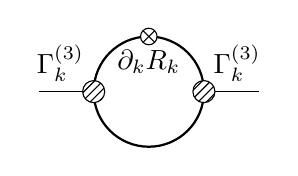
\begin{tikzpicture}
  \draw[thick] (0,0) circle (\unit);
  \draw (-2*\unit,0) -- (-\unit,0) (\unit,0) -- (2*\unit,0);
  \draw[fill=white,cross] (0,\unit) circle (0.15*\unit) node[below=2*\unit] {$\partial_k R_k$};

  \draw[fill=white,postaction={pattern=north east lines}] (\unit,0) circle (0.2*\unit) node[above right] {$\Gamma_k^{(3)}$} (-\unit,0) circle (0.2*\unit) node[above left] {$\Gamma_k^{(3)}$};
\end{tikzpicture}

% Diagram 2
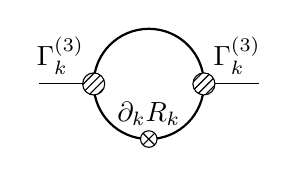
\begin{tikzpicture}
  \draw[thick] (0,0) circle (\unit);
  \draw (-2*\unit,0) -- (-\unit,0) (\unit,0) -- (2*\unit,0);
  \draw[fill=white,cross] (0,-\unit) circle (0.15*\unit) node[above=2*\unit] {$\partial_k R_k$};

  \draw[fill=white,postaction={pattern=north east lines}] (\unit,0) circle (0.2*\unit) node[above right] {$\Gamma_k^{(3)}$} (-\unit,0) circle (0.2*\unit) node[above left] {$\Gamma_k^{(3)}$};
\end{tikzpicture}

% Diagram 3
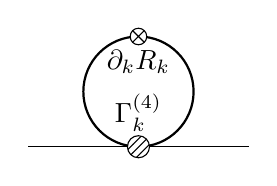
\begin{tikzpicture}
  \draw[thick] (0,0) circle (\unit);
  \draw (-2*\unit,-\unit) -- (2*\unit,-\unit);
  \draw[fill=white,cross] (0,\unit) circle (0.15*\unit) node[below=2*\unit] {$\partial_k R_k$};

  \draw[fill=white,postaction={pattern=north east lines}] (0,-\unit) circle (0.2*\unit) node[above=3*\unit] {$\Gamma_k^{(4)}$};
\end{tikzpicture}

\end{document}
